% Anonymous author-review draft. Results are generated only after completed-run verification.
\documentclass[runningheads]{llncs}
\usepackage[T1]{fontenc}
\usepackage{amsmath,amssymb,graphicx,booktabs,xurl,placeins}
\usepackage[hidelinks]{hyperref}
\urlstyle{rm}
\hypersetup{pdfauthor={},pdftitle={History-Conditioned SAC under Sensor Faults: A Pilot Study of Adaptation and Retention},pdfsubject={Anonymous conference author-review draft},pdfkeywords={reinforcement learning, sensor faults, adaptation, retention, experience replay}}
\begin{document}
\title{History-Conditioned SAC under Sensor Faults: A Pilot Study of Adaptation and Retention}
\titlerunning{Adaptation and Retention under Sensor Faults}
\author{Anonymous Author(s)}
\authorrunning{Anonymous submission}
\institute{}
\maketitle

\begin{abstract}
Adapting during training while retaining earlier behavior requires measuring both outcomes. We report a warm-start pilot of history-conditioned Soft Actor-Critic under incorrect or delayed observations in HalfCheetah-v5. Three pretrained transformer policies and three reactive policies each branch into observation noise or a three-step delay, with either no retained replay or a 50\% mixture of earlier clean-condition experience. All 24 branches receive 4,000 new-condition interactions and matched update counts. The same updated model is evaluated on both the sensor condition and the original clean condition. Without retained replay, mean delay-condition return improves by 98.1 for the transformer and 383.7 for the reactive controller, while clean-condition return declines by 825.4 and 1,158.9, respectively. With retained replay, those clean-condition declines are 145.2 and 383.9, but delay-condition gains fall to 10.2 and 228.2. Mean noise-condition performance declines in all four controller/replay combinations. Every branch loses measured clean-condition performance. Saved trajectories verify actual observation corruption, and checkpoint audits verify paired initialization and same-model retention measurement. These short-budget, three-seed results expose an adaptation--retention tradeoff in the tested configuration; they do not establish fast adaptation without forgetting or a general advantage of history conditioning.

\keywords{Reinforcement learning \and Sensor faults \and History conditioning \and Retention \and Experience replay}
\end{abstract}

\section{Introduction}
An adaptive controller should learn to operate under new conditions while preserving useful behavior acquired earlier. Rapid improvement on a new task and retention of an old task are separate requirements: a policy can improve on one while deteriorating on the other. Our long-term research objective is to combine these capabilities in real-time control. During development of an SAC-based controller, training plateaus in experiments with transformer and world-model-style components motivated a more controlled investigation of how recent interaction history and retained experience affect adaptation. Those development observations motivate this study; they are not a matched architectural comparison or evidence of a diagnosed cause of the plateaus.

A plateau must also be distinguished from forgetting. A model that stops improving has not necessarily lost previously acquired behavior. Conversely, continued improvement on current data can conceal deterioration on earlier conditions. Work on primacy bias identifies an influence of early experience on later reinforcement learning (RL)~\cite{primacy}, while research on plasticity examines a model's continuing ability to learn~\cite{plasticity}. These provide relevant context, but neither mechanism can be assigned to a particular stalled run without an appropriate measurement. We therefore measure new-condition performance and old-condition retention directly, rather than infer either from training loss.

The intended intervention here is a change in sensing. A sensor fault alters what the policy observes: a reading may be noisy or may describe an earlier state. An actuator fault instead alters the applied control. These interventions can create different information requirements even when both reduce return. An earlier benchmark in our development process altered actions; inspection revealed that its sensor-noise label did not implement observation corruption. The present experiment uses a separately verified observation wrapper, and the earlier actuator results are not relabeled as sensor evidence.

History conditioning supplies a policy with a sequence of observations, actions, and rewards. A transformer is one way to encode that information, while Soft Actor-Critic (SAC) supplies a learning objective~\cite{sac}. These are complementary design choices. In-context RL uses history to change behavior with fixed parameters, as illustrated by RL\textsuperscript{2}~\cite{rl2} and subsequent sequence-based methods~\cite{amago,ad}. Our present question concerns \emph{continued parameter learning}: after a trained controller encounters changed sensing, does further training improve its return, and what happens to its earlier clean-condition performance?

We conduct an explicitly bounded pilot in HalfCheetah-v5. Three existing checkpoints per architecture initialize a history-conditioned transformer and a reactive controller. Each checkpoint branches into two sensor conditions and two replay strategies. Both strategies receive the same new-condition interaction and update budgets; one also samples a fixed pool of earlier clean-condition experience. We evaluate the same updated model on the new and old conditions at fixed budgets. The resulting 24 branches are derived from six source models, not 24 independent training seeds.

This study contributes (i) an implemented and behaviorally verified sensor-fault intervention; (ii) a paired continued-training comparison with explicit adaptation and retention measurements; and (iii) an auditable record of the experiment's limits. It does not propose a new general-purpose algorithm, establish adaptation to arbitrary new environments, or equate a short pilot with a solution to forgetting.

\subsection{Related Work}
\paragraph{Memory and adaptation.}
Recurrent model-free policies can be strong baselines in partially observed tasks when their design and training are carefully controlled~\cite{ni}. AMAGO studies off-policy transformer-based in-context RL~\cite{amago}, and AMAGO-2 addresses multi-task learning across differing return scales~\cite{amago2}. Algorithm Distillation learns from algorithm-generated learning histories~\cite{ad}. Our much smaller configuration uses a conventional critic-regression objective and directly collected experience. It does not reproduce those complete methods or evaluate their task breadth. Its history resets between episodes; continued parameter updates supply the cross-episode adaptation examined here.

\paragraph{Replay and retention.}
CLEAR combines replay with additional learning objectives to address stability and plasticity in continual RL~\cite{clear}. RLPD studies efficient online RL using prior data~\cite{rlpd}. These findings motivate testing retained experience, but they do not imply that an arbitrary old/new replay mixture prevents forgetting. Our intervention changes the source of half of each update batch. It does not implement CLEAR's behavioral-cloning objective or compare against a full RLPD implementation. We report its effect on both evaluation conditions.

\paragraph{Optimization and empirical design.}
The pilot inherits a REDQ-style critic ensemble~\cite{redq} from the existing SAC controllers. DroQ and CrossQ illustrate that normalization and update scheduling can affect learning efficiency~\cite{droq,crossq}. Primacy bias and loss of plasticity provide further reasons to examine the complete learning process~\cite{primacy,plasticity}. None of these mechanisms is separately ablated here. Following empirical-design principles~\cite{empirical}, we fix budgets, retain all specified seeds, expose the initial performance of each branch, and distinguish descriptive seed variation from a formal test of equivalence or no forgetting.

\section{Method}
\subsection{Environment and Sensor Intervention}
We use HalfCheetah-v5 through Gymnasium~\cite{gym}, with 17 observation coordinates, six continuous control dimensions, and a 1,000-step episode horizon. The default observation contains eight position coordinates, excluding absolute horizontal position, followed by nine velocities. The action bounds are $[-1,1]$ in each dimension. Condition $A$ uses unmodified observations. Two separate choices of condition $B$ alter sensing while preserving the requested control and base reward function.

For noise, the policy receives
\begin{equation}
 o_t=s_t+\epsilon_t,\qquad
 \epsilon_{t,j}\sim\mathcal{N}(0,\sigma_j^2),
\end{equation}
independently across coordinates and steps, where $\sigma_j=0.1$ for the eight position coordinates and $\sigma_j=0.5$ for the nine velocities. These values are in native observation units; no normalizer is fitted using evaluation data. A separate seeded generator produces the corruption so that sensor draws do not change the environment's reset randomness.

For delay, the policy receives $o_t=s_{t-3}$. Before three prior steps are available, the sensor vector is zero. The FIFO queue resets at each episode boundary. Both sensor conditions begin at episode reset and remain active throughout the episode. They are known, fixed study conditions; this pilot is not a meta-test over a previously unobserved distribution of sensor mechanisms or severities.

The model input is
\begin{equation}
 x_t=[o_t,a_{t-1},r_{t-1},d_{t-1}]\in\mathbb{R}^{25}.
 \label{eq:input}
\end{equation}
The command and reward fields retain their current timing; only the base sensor vector is corrupted or delayed. All preceding-action, reward, and termination fields are zero at reset. The final flag denotes environment termination rather than time-limit truncation. True sensor readings are saved for verification but are excluded from the policy input and loss. Thus, the experiment concerns faults in the state-observation channel, not simultaneous corruption of every information source.

\subsection{Source Policies and Context Support}
The source models are the validation-selected checkpoints for training seeds 42--44 from an earlier actuator-perturbation study. That study trained on action scaling and action noise; it did not train on these observation faults. The present experiment does not reconstruct those historical training runs. Source checkpoint hashes and the compatible model definitions are captured before this pilot. Condition $A$ is a clean evaluation condition on which these pretrained models already have measurable performance; it is not the result of a new clean-only pretraining phase.

The transformer maps each packed token through a multilayer embedding with LayerNorm and GELU into 64 features. Two causal transformer blocks use two attention heads each and a feed-forward width of 128. Learned absolute positional embeddings provide 128 positions. An eight-dimensional task embedding is concatenated with the transformer output. The actor has two 128-unit hidden layers; each of ten critic heads has two 256-unit hidden layers with LayerNorm. A classifier inherited from the source model is unused: there is no auxiliary fault-label loss in this pilot.

The reactive baseline has a two-layer, 256-unit Gaussian actor and ten two-layer, 256-unit LayerNorm critics. It receives the same 25-dimensional token from Eq.~\ref{eq:input}. Consequently, it retains access to the previous command and reward even though it has no accumulated sequence state. Architectural capacity and preprocessing differ; comparisons between the two controllers do not isolate memory as a single causal factor.

The earlier transformer implementation trained on 32-token windows but could collect and evaluate with 64 tokens. The new pilot restricts collection and evaluation to a rolling queue of at most 32 tokens before any initial or final measurement. Replay reconstructs exactly the corresponding current and successor histories for each sampled transition. A full successor context slides by one token, while an episode-start context grows until it reaches the cap. Right padding follows all valid tokens; causal attention prevents the queried token from attending to that padding.

Each sampled history supervises its final valid transition. With probability 0.25, the replay sampler selects a transition from the first up-to-32 transitions of an episode; otherwise it selects uniformly over the episode. Final transitions are eligible, and an actual successor observation is retained for time-limit bootstrapping. These choices support both short deployment contexts and mature rolling histories. Positions beyond 31 remain unused. The experiment therefore changes the sequence-training implementation as well as the environmental intervention; it is not a replication of the earlier result under a new label.

\subsection{Paired Adaptation and Retained Replay}
For each source model, we first collect two deterministic clean-condition episodes, giving 2,000 old-condition transitions. This fixed pool is shared by all descendant branches of that model. It is distinct from the evaluation episodes. Both replay variants incur the same old-data collection; only the retained-replay variant uses the pool for updates.

Each source model then initializes four independent branches: noise or delay, crossed with old-replay fraction $\rho\in\{0,0.5\}$. Optimizers and entropy temperature are reset identically at each branch because their historical states were not stored in the source checkpoints. Parameters are updated during adaptation. A branch collects four stochastic-policy episodes in condition $B$, totaling 4,000 new-environment steps. After each episode it performs 250 critic-ensemble and actor update cycles. A batch has 64 supervised transitions: all new-condition samples for $\rho=0$, or exactly 32 old and 32 new samples for $\rho=0.5$. Sampling uses replacement from the available episode pools. The same adaptation seed and environment-reset schedule are used for paired replay variants; their trajectories can diverge as their policies change.

For each critic update, the target uses the current actor's next action and the minimum of two randomly selected target critics from the ensemble of ten. The discount is 0.99. Critic losses are summed over the ensemble. The actor minimizes the entropy-adjusted negative value using critics 1 and 2. Transformer features are detached for the actor update; critic regression updates the shared representation. Target encoders and critics use Polyak retention 0.995. Dropout is disabled consistently in collection, evaluation, and fine-tuning; this does not disable gradient computation. No fault identifier is used for training.

\begin{table}[t]
\caption{Fixed pilot configuration. Budgets exclude the earlier source-model training.}
\label{tab:config}
\centering\small
\begin{tabular}{@{}p{0.56\textwidth}p{0.36\textwidth}@{}}
\toprule
Setting & Value \\
\midrule
Pretrained seeds per architecture & 3 (42, 43, 44) \\
Sensor conditions; replay fractions & 2; $0$ or $0.5$ \\
New-condition steps per branch & 4,000 \\
Clean replay collected per source model & 2,000 transitions \\
Batch size; ensemble critics & 64 transitions; 10 \\
Critic-ensemble / actor updates per branch & 1,000 / 1,000 \\
Actor / critic / temperature learning rates & $10^{-4}$ / $10^{-4}$ / $3\!\times\!10^{-4}$ \\
Initial entropy temperature; target entropy & $0.1$; $-6$ \\
Discount; target retention; gradient clip & $0.99$; $0.995$; $10$ \\
Evaluation budgets & 0, 2,000, 4,000 steps \\
Evaluation episodes per condition and budget & 3 deterministic episodes \\
\bottomrule
\end{tabular}
\end{table}

There is one critic-ensemble update per actor update and 0.25 of each per newly collected environment step. The pilot therefore differs from the original source-model update schedule. Each transformer replay sample trains one valid transition, rather than all positions of a sequence; its context still carries a computational cost. Table~\ref{tab:config} records the settings. The run environment is Python 3.12.10, PyTorch 2.11.0 with CUDA 12.8, Gymnasium 1.3.0, and MuJoCo 3.12.0 on Windows with an NVIDIA GeForce RTX 5070 Laptop GPU. Action inference is on CPU and parameter updates are on GPU.

\subsection{Adaptation and Retention Measurements}
At budgets $n\in\{0,2000,4000\}$, we evaluate both $A$ and $B$ using the same checkpoint. Parameters are frozen during evaluation, and context resets each episode. Every condition uses three matched environment seeds, $860000+100e$ for $e=0,1,2$. These episodes never enter replay. Evaluation RNG state is isolated from the training RNG. Checkpoints are retained at fixed budgets; neither sensor performance nor retention determines checkpoint selection.

Let $R^A_{i,c,\rho}(n)$ and $R^B_{i,c,\rho}(n)$ denote mean evaluation returns for source seed $i$, sensor condition $c$, replay fraction $\rho$, and adaptation budget $n$. We report
\begin{align}
 \Delta^B_{i,c,\rho}(n)&=R^B_{i,c,\rho}(n)-R^B_{i,c,\rho}(0),\\
 \Delta^A_{i,c,\rho}(n)&=R^A_{i,c,\rho}(n)-R^A_{i,c,\rho}(0).
\end{align}
A positive new-condition change indicates improved return within the tested budget. A negative old-condition change indicates a loss in measured clean-condition performance. Retention always uses the updated model; restoring the earlier checkpoint would invalidate that comparison.

We also compute a trapezoidal average of $R^B(n)$ over the sampled 0--4,000-step learning curve and paired differences between replay variants. Adaptation elapsed time includes collection and optimization but excludes evaluation and checkpoint I/O. No recovery threshold or acceptable retention-loss margin was specified, so we do not report time to recovery or claim equivalence to the old performance. The three training seeds, rather than their repeated evaluation episodes or descendant branches, are the replication units. We retain every seed and report descriptive means and ranges. Shaded ranges in figures are not confidence intervals.

\subsection{Implementation Verification and Evidence Capture}
Eleven behavioral tests check sensor corruption, timing, random-stream separation, replay boundaries, masking, parameter updates, and positional support. A real MuJoCo test applies identical commands under clean, noisy, and delayed observations and requires identical underlying states and rewards. This verifies that the intervention acts on sensing. A separate short execution check exercises all eight architecture/fault/replay combinations using reduced horizons; those returns are excluded from the pilot analysis.

The pilot snapshots its exact source files, configuration, package versions, and input hashes before collection. Every evaluation records commands, model-input observations, audit-only true observations, sensor ages, rewards, and checkpoint hashes. An independent readback recomputes returns, checks that delayed readings match the recorded earlier states, verifies paired initial performance, and confirms that the same model was used for $A$ and $B$ at each budget. Original source-checkpoint hashes are checked again at completion. This captures the new experiment's provenance without claiming to reconstruct the incomplete historical source capture of pretraining.

\section{Results}
\subsection{Completed Runs and Initial Performance}
All 24 specified branches completed the fixed budget. Separate readback verified 432 evaluation episodes and 48 saved candidate checkpoints, with the six original source checkpoints unchanged. Paired replay variants produced identical initial evaluation returns. The complete study, including clean replay collection, evaluation, checkpoint writing, and initialization, took 1,463.8 seconds on the recorded machine. Table~\ref{tab:outcomes} gives the equally weighted mean over the three source seeds; returns are environment reward sums, not completion rates.

\begin{table}[t]
\caption{Fixed-budget pilot outcomes, averaged equally across three source seeds. $B(0)$ and $B(4000)$ are new-condition returns before and after adaptation; $\Delta A$ is the old clean-condition return change. Returns are not success percentages.}
\label{tab:outcomes}
\centering\small
\begin{tabular*}{\textwidth}{@{\extracolsep{\fill}}llrrrr@{}}
\toprule
Controller & Fault & $\rho$ & $B(0)$ & $B(4000)$ & $\Delta A$ \\
\midrule
Transformer & Noise & 0 & 2433.7 & 2130.1 & $-320.9$ \\
Transformer & Noise & 0.5 & 2433.7 & 2105.1 & $-272.4$ \\
Transformer & Delay & 0 & -85.5 & 12.6 & $-825.4$ \\
Transformer & Delay & 0.5 & -85.5 & -75.3 & $-145.2$ \\
Reactive & Noise & 0 & 2875.5 & 2369.7 & $-641.2$ \\
Reactive & Noise & 0.5 & 2875.5 & 2727.3 & $-339.0$ \\
Reactive & Delay & 0 & -180.3 & 203.4 & $-1158.9$ \\
Reactive & Delay & 0.5 & -180.3 & 47.9 & $-383.9$ \\
\bottomrule
\end{tabular*}
\end{table}


The initial clean-condition means were 2,677.9 (transformer) and 3,328.1 (reactive). The zero-step sensor conditions differed substantially. Mean noise-condition return was 2,433.7 for the transformer and 2,875.5 for the reactive controller. Under the three-step delay, the corresponding means were $-85.5$ and $-180.3$. These are measurements after applying the sensor intervention and before continued training. Different initial performance and source-policy quality constrain cross-controller interpretation.

\subsection{Adaptation under Noise and Delay}
Figure~\ref{fig:adaptation} shows the fixed-budget learning curves. Under noise, mean return declined for both controllers with either replay strategy. Transformer return changed by $-303.7$ without retained replay and $-328.7$ with it. Reactive return changed by $-505.8$ and $-148.2$, respectively. Thus, continued training did not yield a mean noise-condition improvement within this budget, even though the reactive retained-replay arm declined less.

\begin{figure}[!htbp]
\centering
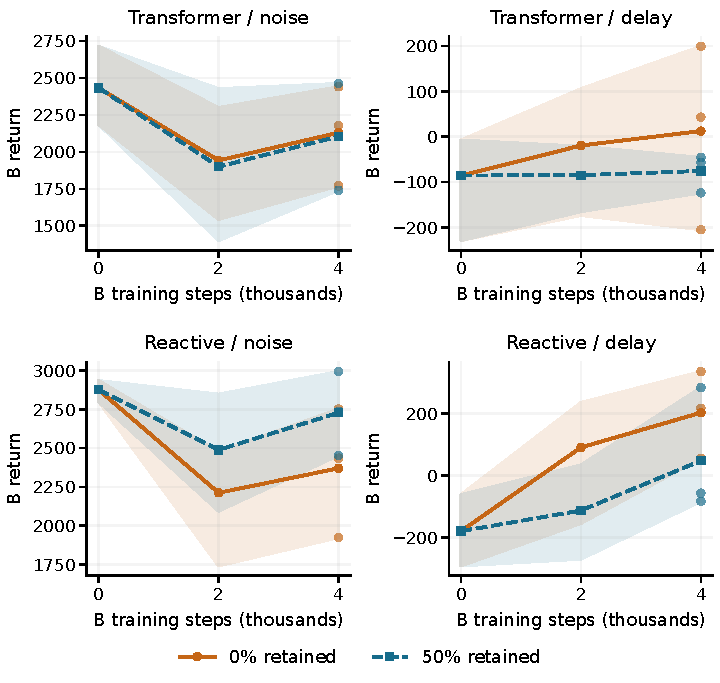
\includegraphics[width=\textwidth]{sensor_adaptation.pdf}
\caption{New-condition return during continued training. Lines are means over three source seeds; shaded bands are their minimum--maximum ranges, not confidence intervals. Small points at the final budget show individual seed means. Evaluation uses three deterministic episodes per seed and condition.}
\label{fig:adaptation}
\end{figure}

Delay produced positive mean changes but substantial variation. Without retained replay, the transformer gained 98.1 return units and the reactive controller gained 383.7. With retained replay, the corresponding gains were 10.2 and 228.2. The transformer's no-replay seed-level changes ranged from $-197.9$ to $+428.8$; its retained-replay changes ranged from $-38.4$ to $+105.4$. Only two of three transformer seeds improved without replay, and one of three improved with replay. All three reactive seeds improved under delay in both replay variants. These counts describe this pilot's realized seed outcomes, not estimated population success probabilities.

The trapezoidal mean return across the sampled learning curve was $-27.8$ without replay and $-82.6$ with replay for transformer delay, compared with 51.2 and $-89.8$ for reactive delay. This summary includes intermediate deterioration that a final-point comparison would hide. It does not establish a recovery time because no recovery threshold was specified.

\subsection{Retention and Paired Replay Effects}
Every branch had a negative clean-condition change at the final budget (Fig.~\ref{fig:retention}). For transformer delay, the mean loss was 825.4 without retained replay and 145.2 with replay. For reactive delay, it was 1,158.9 and 383.9. The corresponding noise-condition adaptation branches lost 320.9 versus 272.4 for the transformer and 641.2 versus 339.0 for the reactive controller.

\begin{figure}[!htbp]
\centering
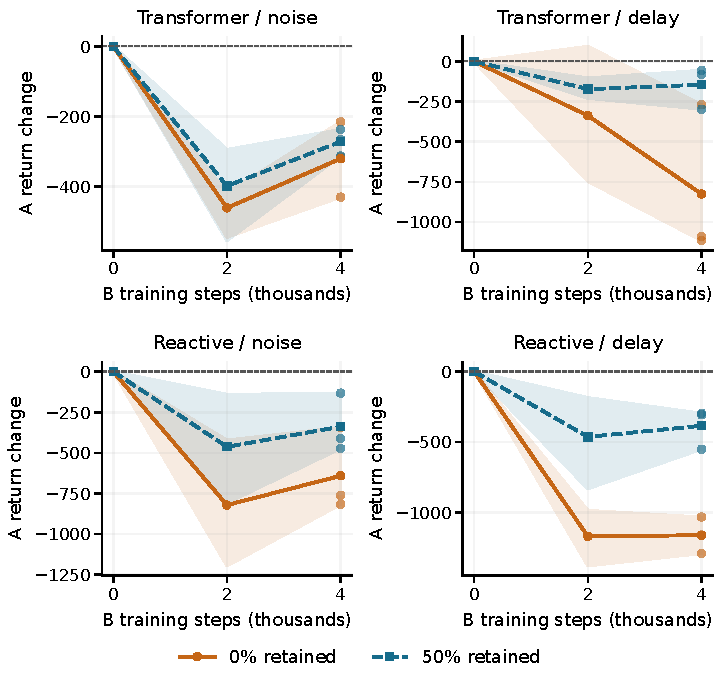
\includegraphics[width=\textwidth]{sensor_retention.pdf}
\caption{Clean-condition retention measured with the actual updated model. Zero is each branch's own initial clean-condition return. Negative values indicate loss of earlier measured performance. Lines and shaded ranges summarize three source seeds; the ranges are not confidence intervals.}
\label{fig:retention}
\end{figure}

Retained replay increased final clean-condition return relative to the paired no-replay branch in ten of twelve seed/controller/fault pairs. Its mean effect on clean return was positive in all four controller/fault comparisons. This was not uniform at the seed level: transformer seed 43 under noise and seed 42 under delay retained less with replay. For both controllers, all three delay seeds ended with lower delay-condition return under retained replay than under no replay. The paired comparison therefore exposes a cost in new-condition performance alongside improved average retention under delay. Neither arm preserved its own initial clean performance.

Mean collection-and-optimization time per branch ranged from 55.1 to 75.0 seconds across transformer conditions and from 34.9 to 38.3 seconds across reactive conditions. Those times exclude evaluation and checkpoint I/O. They describe this implementation and machine load; they do not establish equal computational budgets or a generally faster adaptation algorithm.


\FloatBarrier
\section{Discussion}
The pilot makes the distinction between adaptation and retention observable. A controller can gain return under delayed sensing while losing performance with clean observations. Under delay, mixing earlier experience into the update batch reduced the average clean-condition loss for both controllers, but also reduced their mean new-condition gain. The tested replay mixture therefore trades one measured outcome against the other; it does not satisfy the original objective of rapid adaptation with preserved earlier behavior.

Noise and delay also require separate interpretation. The source policies already obtained comparatively high returns under the chosen noise level, whereas delay caused much lower initial returns. Further training reduced average noise-condition return, so more interaction and gradient updates were not sufficient to improve that condition within this budget. Under delay there was more room for improvement, yet transformer outcomes differed in sign across seeds. Pooling the faults into one headline score would obscure these distinctions.

The comparison does not demonstrate that history is inherently ineffective. It compares particular pretrained controllers whose capacities, representations, and initial outcomes differ. Aligning context support removes a known implementation inconsistency, but it cannot by itself ensure a useful learned representation or stable continued learning. The reactive controller's larger mean delay gain is evidence about these tested configurations, not a controlled causal estimate of the value of memory.

Likewise, the observed clean-condition declines should not be assigned to a single mechanism. They occur after training on changed sensing, but optimizer resets, source-policy quality, representation updates, and the narrow retained pool may also influence the result. A continued-clean-training control is needed to quantify deterioration caused by continued optimization alone. Primacy bias or loss of plasticity remain possible topics for subsequent diagnosis, rather than explanations established by these measurements. The practical outcome of this pilot is a verified experimental basis for that diagnosis and a clear requirement to evaluate old and new conditions together.


\subsection{Limits of the Pilot}
The source checkpoints were trained with actuator perturbations, and the clean condition is an evaluation setting rather than a newly optimized clean-only task. Adapting these models may differ from training a sensor-aware agent from scratch. Optimizers and entropy temperature are reinitialized; this may itself influence continued learning. The current pilot cannot separate that effect from sensitivity to the new observation distribution. Both replay variants share that initialization, which supports their within-model comparison but does not remove the limitation.

The retained pool contains only two deterministic clean episodes per model. It covers a narrow part of the old state distribution and contains no explicit behavioral-cloning or feature-preservation loss. Half of a batch drawn from this pool is a particular rehearsal strategy, not a general guarantee of retention. The two architectures also differ in capacity, input processing, and pretraining outcomes. Three seeds and three fixed evaluation episodes per condition provide a limited basis for generalization. Averages may conceal opposite outcomes across source models; the released tables retain the seed-level values.

This is a single locomotion environment with two fixed sensor conditions, one delay, one noise vector, and a 4,000-step adaptation budget. It does not measure arbitrary new-map transfer, visual sensing, unknown fault onset during deployment, changing severity, or long sequences of tasks. The model retains a current reward and command channel, so its information loss is narrower than complete sensor failure. No longer-budget plateau, recovery threshold, or retention tolerance is inferred from the three recorded evaluation budgets. We report realized pilot behavior rather than declare that fast adaptation without forgetting has been achieved.

\subsection{Next Evaluation}
A subsequent study should specify acceptable old-task degradation and a new-task recovery criterion before final evaluation. It should include more independent source models and evaluation states, a longer budget, multiple task orders, and a baseline that continues training on $A$ for the same number of updates. That continuation control would help distinguish general fine-tuning instability from changes specific to $B$. A matched context encoder and parameter budget would improve architectural attribution.

The retention mechanism also warrants a controlled comparison: ordinary replay, retained replay, and an explicitly defined behavioral or feature anchor should share the same new-data budget. Data selection and source-policy quality should be varied separately. Any resulting candidate must still be evaluated on the earlier conditions using its actual updated weights. These additions would move the evaluation closer to the original goal while preserving the distinction between learning a new condition, retaining an old one, and remaining capable of future learning.

\section{Conclusion}
We implemented actual sensor noise and observation delay, aligned transformer history support, and completed a paired pilot of continued SAC training with explicit retention measurements. Across three pretrained seeds per controller, retained replay reduced average clean-condition loss in every controller/fault comparison but did not eliminate it. Under delay, improved average retention accompanied smaller new-condition gains; under noise, mean new-condition performance declined in all variants. These findings do not establish fast adaptation without forgetting. They identify the tradeoff exhibited by this configuration and motivate longer, controlled studies of replay coverage, explicit retention objectives, and continued-learning stability.


% Competing interests require factual author confirmation; no unsupported declaration is inserted.
\begin{samepage}
\section*{AI Usage Declaration}
Google Antigravity with a Gemini model assisted implementation of earlier research architecture and algorithms. OpenAI Codex assisted manuscript restructuring, primary-source lookup, formatting, code inspection, implementation and testing of the sensor-fault pilot, experiment orchestration, result verification, and preparation of analysis and plotting scripts. The reported observations were generated by executed simulator runs; tables and figures are computed from saved run records. Generative AI was not used to invent experimental observations. The authors remain responsible for the implementation, source verification, analysis, interpretation, and final manuscript.
\par\end{samepage}
\bibliographystyle{splncs04}
\bibliography{references}
\end{document}
